\section{Chức năng tạo album và đánh dấu bài hát yêu thích}
Người dùng có thể tạo album riêng để lưu trữ các bài hát yêu thích và dễ dàng truy cập lại. Ngoài ra, có thể đánh dấu các bài hát là “Yêu thích” để sắp xếp và lọc nhanh.

\subsection{Chức năng tạo album}
% Chèn hình minh họa tạo album và đánh dấu yêu thích
\begin{figure}[H]
    \centering
    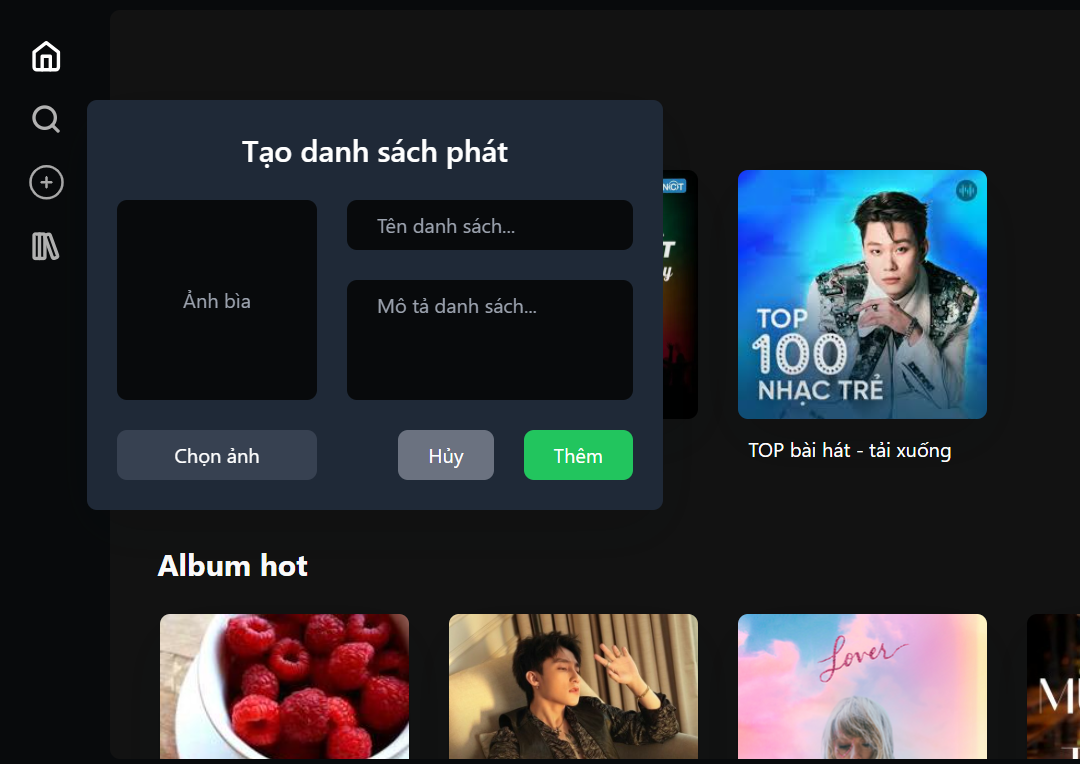
\includegraphics[width=1\textwidth]{imgs/chap5/tao_album_1.png}
    \caption{Giao diện hiện biểu mẫu tạo album}
\end{figure}

\begin{figure}[H]
    \centering
    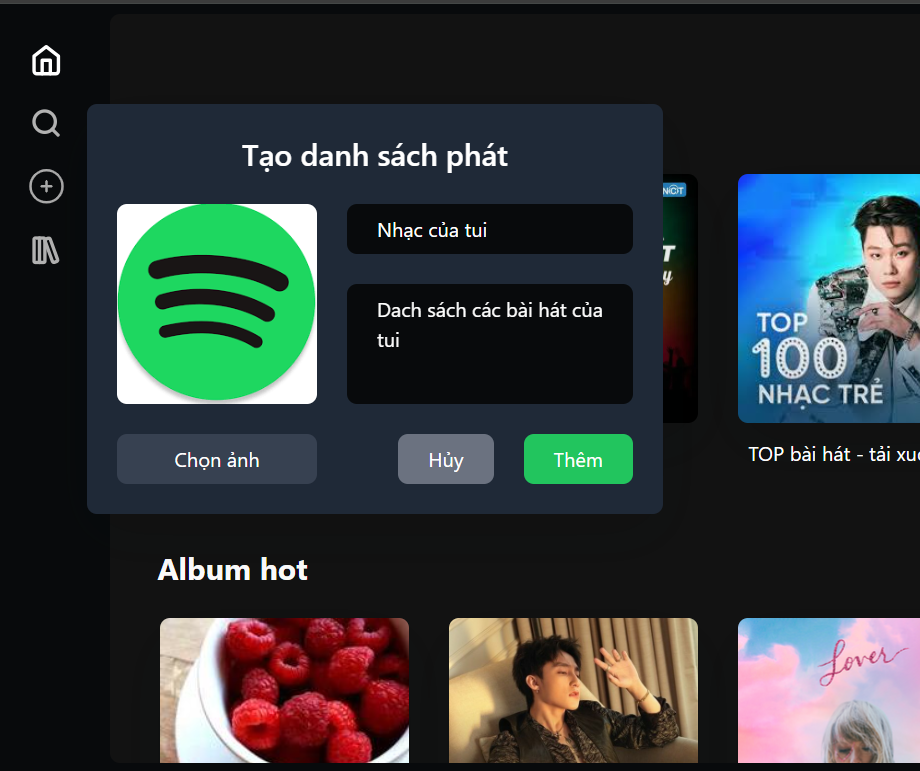
\includegraphics[width=1\textwidth]{imgs/chap5/tao_album_2.png}
    \caption{Giao diện điền thông tin tạo album}
\end{figure}

\begin{figure}[H]
    \centering
    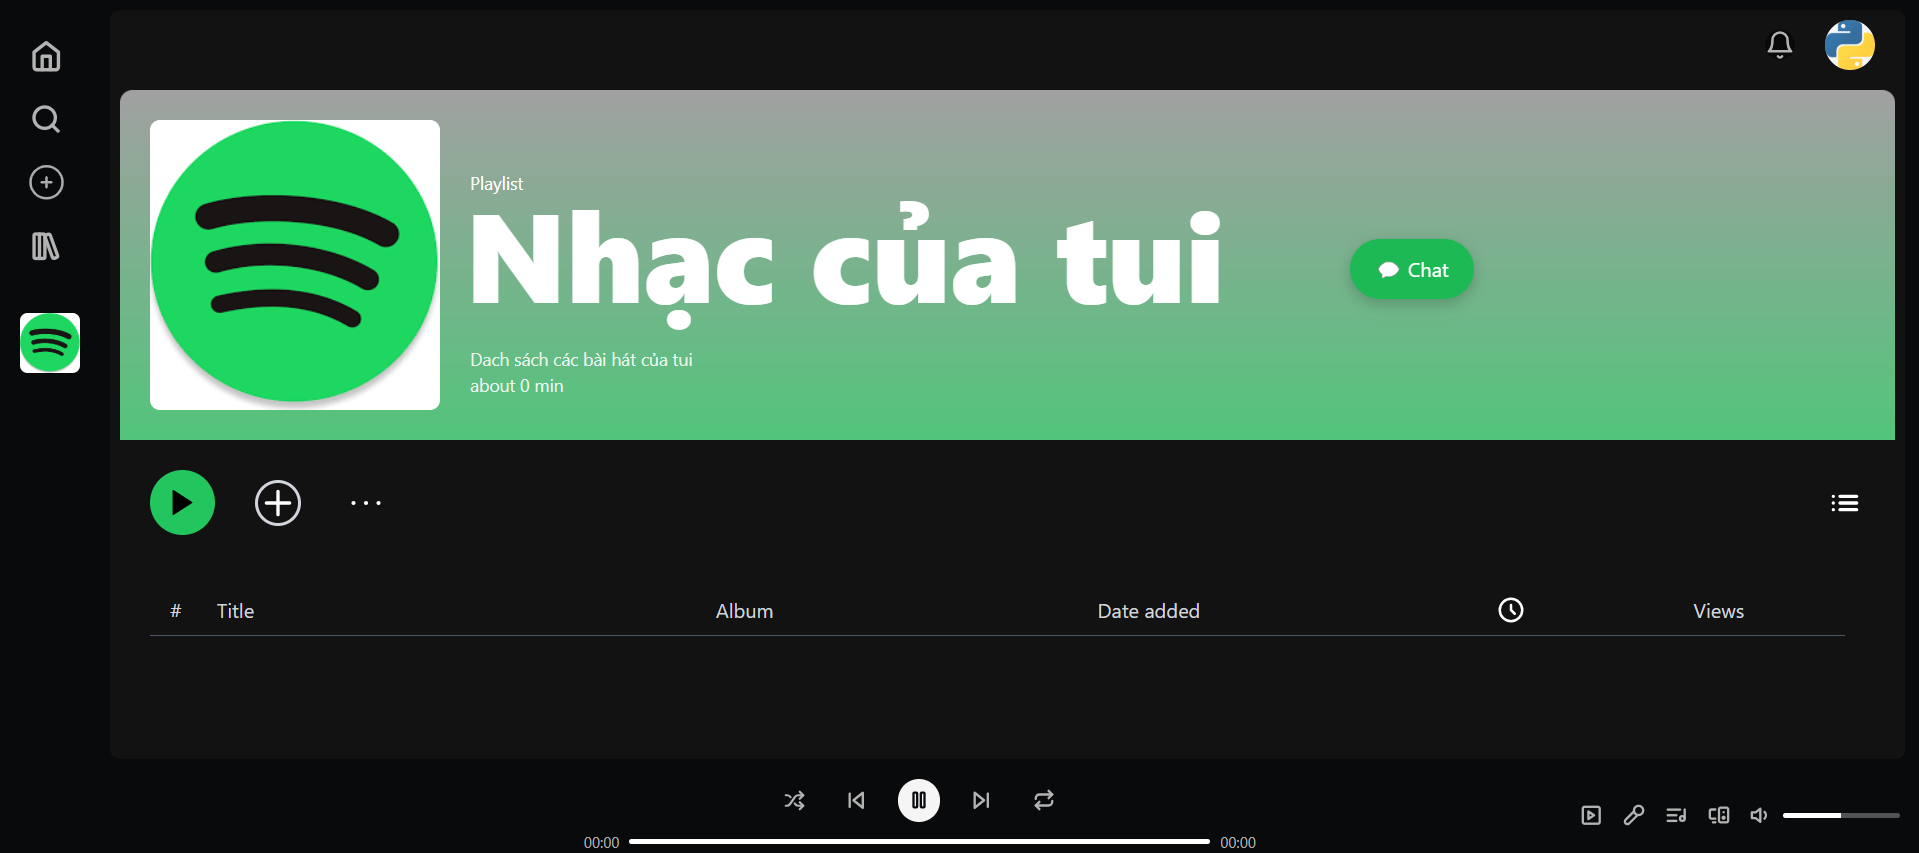
\includegraphics[width=1\textwidth]{imgs/chap5/tao_album_3.png}
    \caption{Giao diện tạo album thành công}
\end{figure}

\begin{figure}[H]
    \centering
    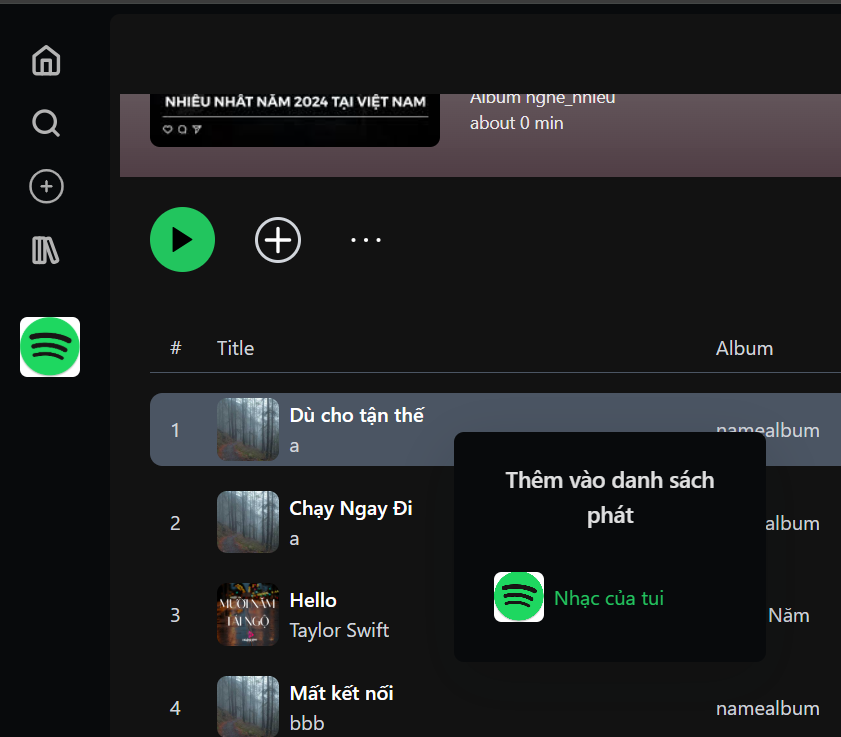
\includegraphics[width=1\textwidth]{imgs/chap5/tao_album_4.png}
    \caption{Giao diện thêm bài hát vào album}
\end{figure}

\begin{figure}[H]
    \centering
    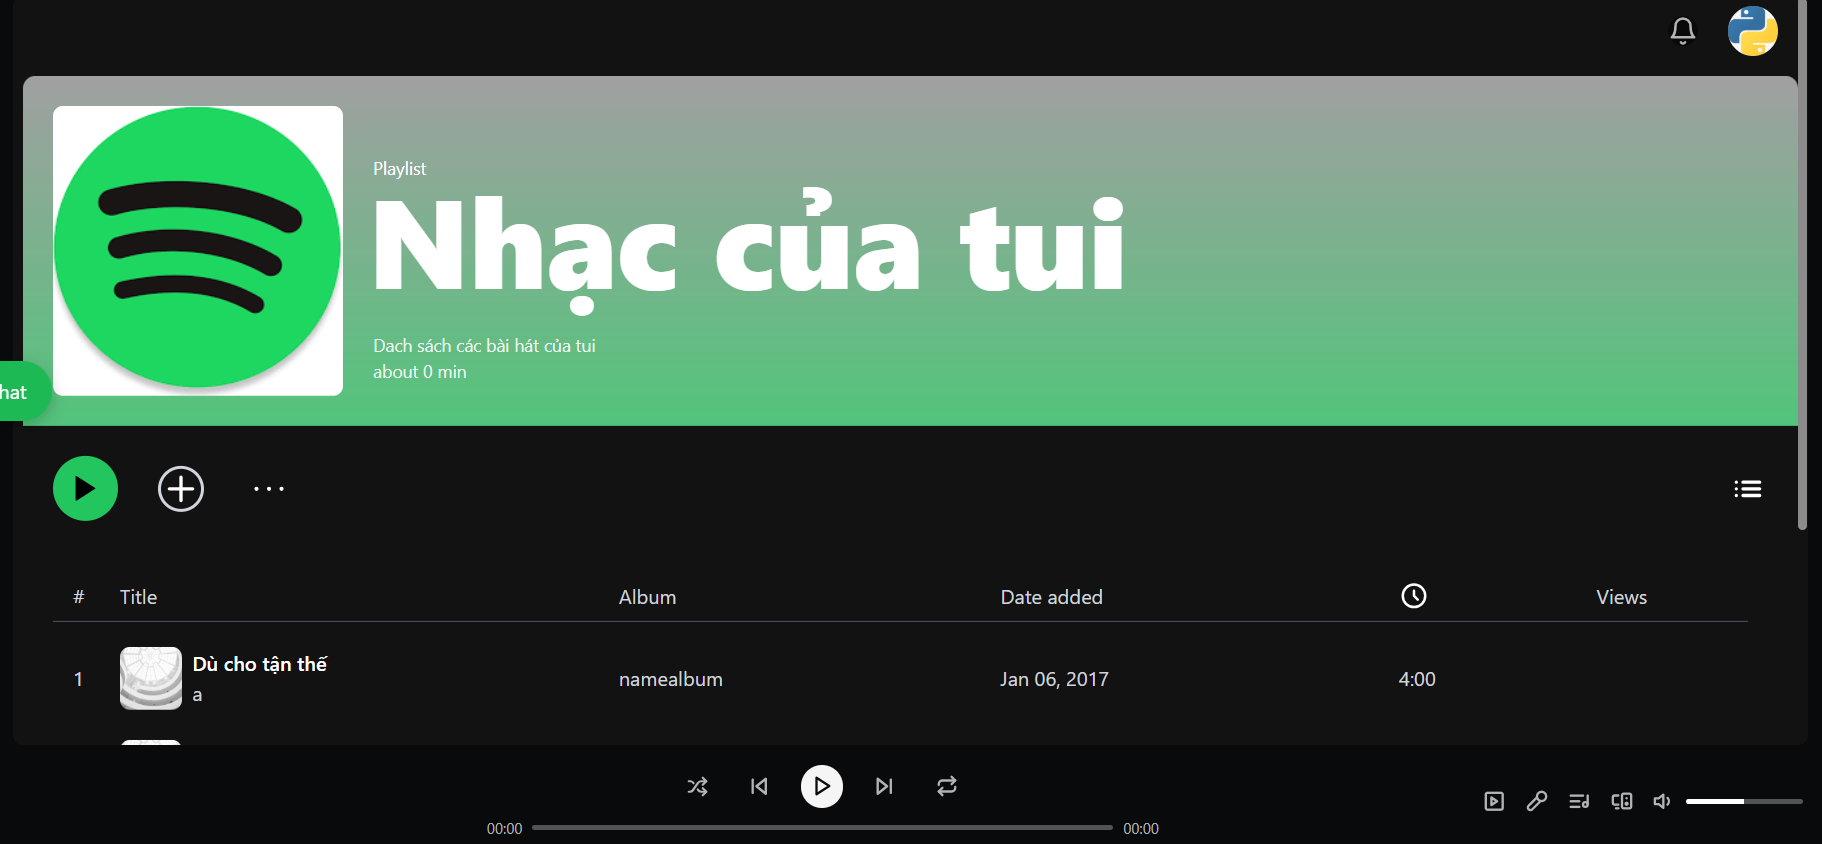
\includegraphics[width=1\textwidth]{imgs/chap5/tao_album_5.png}
    \caption{Giao diện album đã bài hát thành công}
\end{figure}

\subsection{Chức năng đánh dấu bài hát yêu thích}
